\chapter{Paradoxe Hitzeempfindung}\label{appendix:paradoxehitzeempfindung}
\section*{Modellierung von MCP-Netzen unter Berücksichtigung von Zeiteinheiten}

Bislang haben wir nur MCP-Netze betrachtet, bei denen wir die Zeiteinheiten nicht berücksichtigt haben. In Anlehnung an das McCulloch und Pitts-Paper Original-Arbeit wollen wir jetzt ein Netz modellieren, das die \textbf{paradoxe Hitzeempfindung}~\cite{HVKJ82} simuliert: Das Phänomen, das bei kurzzeitiger Kühlung der Haut Hitze empfunden wird.\\

\blockquote[{\cite[106]{MP43}}]{
    If a cold object is held to the skin for a moment and removed, a sensation of heat will be felt; if it is applied for a longer time, the sensation will be only of cold, with no preliminary warmth, however transient.
}\\

Das nach~\cite[105, Figure 1 (e)]{MP43} aufgestellte Modell und die dazugehörige Formel übertragen wir nun in die von uns verwendete Notation (vgl. [Fau94:31 ff.]). In der Abbildung~\ref{fig-mcpheat} sind zwei Temperaturrezeptoren $H_i$ (Hitze) und $K_i$ (Kälte) dargestellt, ausserdem hat das Netz zwei Ausgänge, $H_o$ und $K_o$. $H_o$ wird zum Zeitpunkt $t$ aktiviert, wenn Hitze empfunden wird, $K_o$ entsprechend bei Kälte.
\noindent
Die Bedingungen für eine Aktivierung von $H_o$ lauten: Hitze wird signalisiert, wenn entweder der Wäremerezeptor durch Wärme stimuliert wird \textbf{oder} kurzzeitig ein Kälteimpuls von den Kälterezeptoren registriert wird.\\

Formal dargestellt\footnote{
    s.~\cite[106]{MP43}
}:

\begin{equation}
    H_o(t) \equiv H_i(t-1) \lor (K_i(t-3) \land \neg K_i(t - 2))
    \label{eq:gl-heat}
\end{equation}

Die Bedingungen für eine Aktivierung der Zelle $K_o$, um Kälte zu signalisieren, lautet


\begin{equation}
    K_o(t) \equiv K_i(t-2) \land K_i(t-1)
    \label{eq:gl-cold}
\end{equation}

\begin{figure}[h]
    \centering
    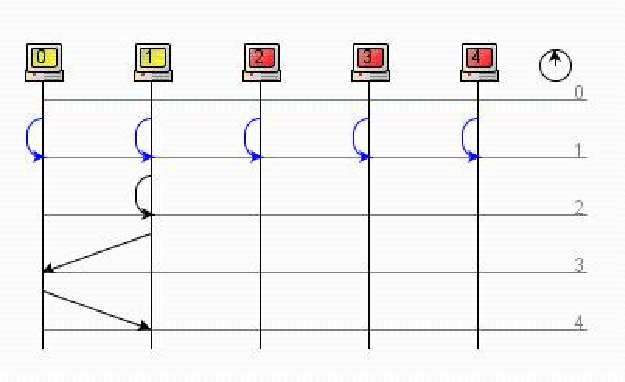
\includegraphics{images/p1ReadSeq.pdf}
    \caption{MCP-Netz zur Modellierung der paradoxen Hitzeempfindung.}
    \label{fig-mcpheat}
\end{figure}

\noindent
Zeitabhängige Werte der MCP-Zellen wollen wir nun durch Formeln auszudrücken.
Die zu dem Zeitpunkt $t$ bekannten Werte sind bereits in Gleichung~\ref{eq:gl-heat} sowie Gleichung~\ref{eq:gl-cold} erfaßt.
\noindent
Es folgt für $H_o(t)$

\begin{equation}
    H_o(t) \equiv Z_1(t-1) \lor H_i(t-1)
    \label{eq:gl-heat1}
\end{equation}
\noindent
Gleichung~\ref{eq:gl-heat1} ist abhängig von $Z_1$ und $H_i$ zum Zeitpunkt $t - 1$. $Z_1(t-1)$ ist trivialerweise der Wert, mit dem der Rezeptor stimuliert wurde. Für $Z_1(t-1)$ folgt:

\begin{equation}
    Z_1(t - 1) \equiv Z_2(t-2) \land \neg K_i(t-2)
    \label{eq:gl-z1}
\end{equation}
\noindent
Analog zu $H_i(t - 1)$ ist $K_i(t - 2)$ einfach der Stimulus für den Rezeptor.
Deshalb benötigen wir nur noch $Z_2(t-2)$, was einfach das efferente Signal von $K_i(t-3)$ erhält:

\begin{equation}
    Z_2(t-2) \equiv K_i(t-3)
    \label{eq:gl-z2}
\end{equation}
\noindent
Die Abfolge der Aktivierung von $K_o$ bzw. $H_o$ kann nun tabellarisch auf Grundlage der Gleichungen dargestellt werden.
Hierbei ist der Inhalt der Tabellenzellen (bis auf die Spalte $t$) $f(g(X))$  (siehe Gleichung~\ref{eq:gl-activation}), sofern der Wert zu dem entsprechenden Zeitpunkt bekannt ist (vgl. [Fau94:32-33]).
\noindent
Wir beginnen mit der Stimulierung von $K_i$ durch zwei aufeinanderfolgende Kälteimpulse (Abbildung~\ref{fig-coldimp}). Tabelle~\ref{tab:coldimp} stellt die die jeweiligen Schritte dar: Es wird erwartet, das $K_o$ feuert. Tabelle~\ref{tab:heatimp} beschreibt im Gegenzug die Erwartung ``Wärme`` an die Ausgabe für einen Stimulus von $H_i$, dargestellt in Abbildung~\ref{fig-heatimp}.

\begin{figure}[h]
    \centering
    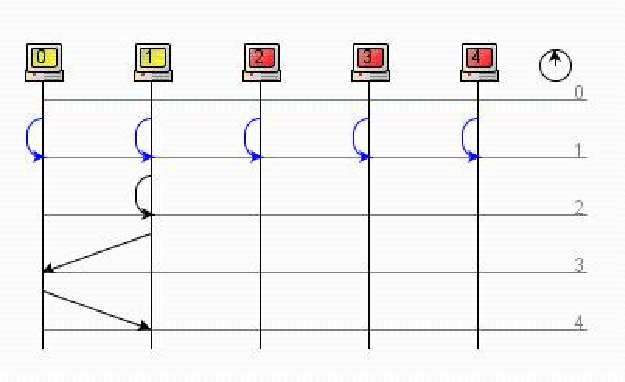
\includegraphics{images/p1ReadSeq.pdf}
    \caption{Zwei Kälteimpulse werden nacheinander in das Netz gespeist.}
    \label{fig-coldimp}
\end{figure}


\begin{table} %[hbtp]
    \centering
    \begin{tabular}{c | c | c | c | c | c | c}
        $t$   & $H_i$ & $K_i$ & $Z_1$ & $Z_2$ & $H_o$ & $K_o$ \\
        \hline
        $t-2$ & 0     & 1     &          &          &          &          \\
        $t-1$ & 0     & 1     & 0        & 1        &          &          \\
        $t$   &       &       & 0         & 1         & 0        & 1        \\
    \end{tabular}
    \caption{Tabellarische Darstellung von zwei Kälteimpulsen}
    \label{tab:coldimp}
\end{table}


\begin{figure}[h]
    \centering
    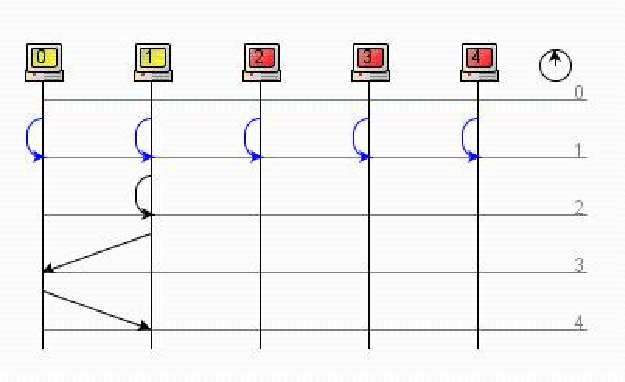
\includegraphics{images/p1ReadSeq.pdf}
    \caption{Ein einzelner Wärmeimpuls aktiviert das Wärmesignal.}
    \label{fig-heatimp}
\end{figure}



\begin{table} %[hbtp]
    \centering
    \begin{tabular}{c | c | c | c | c | c | c}
        $t$   & $H_i$ & $K_i$ & $Z_1$ & $Z_2$ & $H_o$ & $K_o$ \\
        \hline
        $t-1$ & 1     & 0     &          &          &          &          \\
        $t$   &       &       &          & 0         & 1        & 0        \\
    \end{tabular}
    \caption{Tabellarische Darstellung von einem Wärmeimpuls}
    \label{tab:heatimp}
\end{table}



Die Simulation der paradoxen Hitzeempfindung (Abbildung~\ref{fig-heatparad}) erfolgt nun durch eine einmalige Aktivierung von $K_i$ zum Zeitpunkt $t-3$.
Danach wird der Stimulus entfernt: formal wird das durch $\neg K_i (t-2)$ ausgedrückt (s. Gleichung~\ref{eq:gl-heat}).

\begin{table} %[hbtp]
    \centering
    \begin{tabular}{c | c | c | c | c | c | c}
        $t$   & $H_i$ & $K_i$ & $Z_1$ & $Z_2$ & $H_o$ & $K_o$ \\
        \hline
        $t-3$   &  0  &  1  &    &    &    &  \\
        $t-2$   &  0  &  0  &  0  & 1   &    &  \\
        $t-1$   &    &    &   1 & 0   &  0  & 0 \\
        $t$   &    &    &    &    &  1  & 0 \\
    \end{tabular}
    \caption{Tabellarische Darstellung der paradoxen Hitzeempfindung}
    \label{tab:heatparad}
\end{table}

\begin{figure}[h]
    \centering
    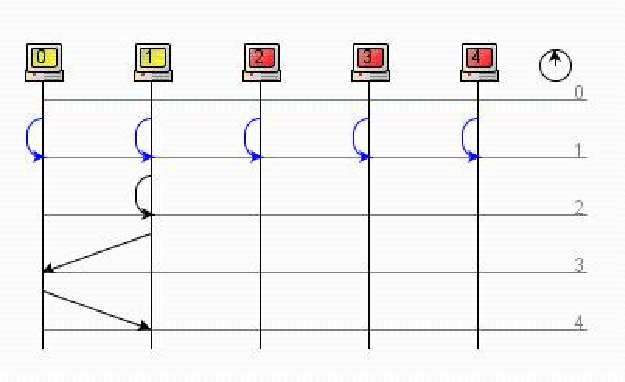
\includegraphics{images/p1ReadSeq.pdf}
    \caption{Die paradoxen Hitzeempfindung durch einen einzelnen Kälteimpuls.}
    \label{fig-heatparad}
\end{figure}
